\documentclass[a4paper,12pt]{article}
\usepackage[a4paper, margin=2cm]{geometry}
\usepackage[utf8]{inputenc}
\usepackage{amsmath, amssymb} % Packages pour les maths
\usepackage[T1]{fontenc}
\usepackage{graphicx} 
\usepackage{caption}
\usepackage{setspace} % Espacement des lignes
\usepackage{tikz}
\usepackage{soul}
\usepackage{titlesec}
\usepackage{hyperref}
\renewcommand{\contentsname}{Table des matières}
\usepackage[colorlinks=true, linkcolor=blue, urlcolor=blue, citecolor=blue]{hyperref}
\titleformat*{\section}{\LARGE\bfseries}
\titleformat*{\subsection}{\Large\bfseries}
\titleformat*{\subsubsection}{\normalsize\bfseries}
\titleformat{\part}[display]
  {\normalfont\Huge\bfseries}{}{0pt}{}
\begin{document}
\begin{titlepage}
    \centering
    \vspace*{3cm}
    {\Huge \textbf{Document de Synthèse}\par}
    \vspace{2cm}
    {\Large Les Carcajous Callypiges\par}
    \vfill
    {\large 2025\par}
\end{titlepage}
\tableofcontents
\newpage
\addcontentsline{toc}{section}{Introduction}

{\LARGE \textbf{Introduction}}
\input{documentation/Evolution du projet CREPES.txt}



\newpage
\section{Modèle 1}
\subsection{Bille remplie d'eau}
\addcontentsline{toc}{subsubsection}{Hypothèses} 
\textbf{Hypothèses}

\begin{itemize}
    \item Terre assimilée à une boule d'eau, de température \(T_{\text{Terre}}\) telle que \(T_{\text{Terre}}\)> \(T_{\text{ext}}\)
    \item  Sans atmosphère (dans le vide)
    \item  Sans puissance solaire reçue  
    \item \(c_{m}= c_{\text{m,eau}} \sim c_{\text{m,Terre}}\) 
    \item $T(t=0) = T_i$ \ \ \
$T(t \to +\infty) = T_0$
   
\end{itemize}
$\rightarrow$ la terre perd de la température par rayonnement
\\ 

\addcontentsline{toc}{subsubsection}{Schéma}
\textbf{Schéma}
\\
\noindent\textcolor{gray}{\rule{\linewidth}{0.4pt}}

    
\begin{center}
  \input{modele1/figures/Schéma mathcha modèle 1.1.txt}
\end{center}



\noindent\textcolor{gray}{\rule{\linewidth}{0.4pt}} 

\vspace{1em}

\addcontentsline{toc}{subsubsection}{Equation}
\textbf{Equation}
\[   P = \sigma T^4 \cdot S
\]

\[    C \, \frac{dT}{dt} = - \sigma T^4 \,  \cdot S
\]

\[\frac{dT}{dt} = - \frac{4 \pi R_T^2 \sigma T^4}{C}\]  

Avec 
\(S= 4\pi r^2\)
\ \ \ \
\(\sigma=5,67 \cdot 10^{-8} W\cdot m^{-2} \cdot K^{-4}\)

\addcontentsline{toc}{subsubsection}{Solution}
\textbf{Solution} 
\[
T(t) = \left( \frac{C}{C/T_i^3 + 12\pi R^2 \sigma t} \right)^{1/3} 
= \frac{T_i}{\left(1 + 3k T_i^3 t \right)^{1/3}}
\]
avec \(k=\frac{4\pi R_T^2 \sigma}{C}\)
et \(C=c_{\text{m eau}}\times m=4,60 \cdot 10^{27} J\cdot K^{-1}\)

\bigskip



\bigskip

\addcontentsline{toc}{subsubsection}{Modélisation graphique}
\textbf{Modélisation graphique} 

\begin{center}
  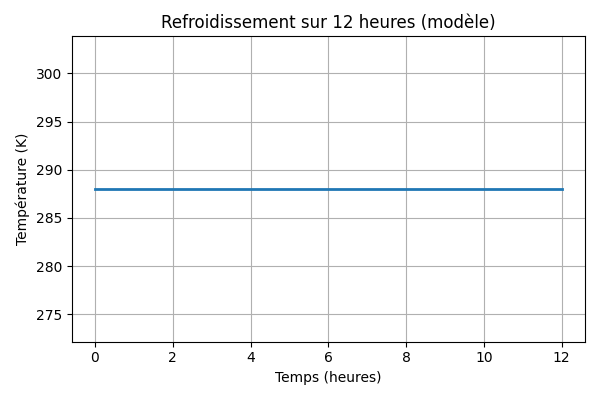
\includegraphics[width=0.8\linewidth]{../modele1/figures/modele1.png}
\end{center}
    
    

\subsection{Coquille vide }
\addcontentsline{toc}{subsubsection}{Hypothèses}
\textbf{Hypothèses}
\begin{itemize}
    \item On garde les hypothèses précédentes, excepté le système: la Terre est assimilée à une coquille d'eau, d'épaisseur dr, qui a un intérieur vide
    
\end{itemize}
$\rightarrow$ il faut donc recalculer la capacité thermique 

\addcontentsline{toc}{subsubsection}{Schéma}
\textbf{Schéma}

\noindent\textcolor{gray}{\rule{\linewidth}{0.4pt}}

    
\begin{center}
  \input{modele1/figures/Schéma modèle 1.2 coquille.txt}
\end{center}



\noindent\textcolor{gray}{\rule{\linewidth}{0.4pt}} 




\addcontentsline{toc}{subsubsection}{Calcul capacité thermique}
\textbf{Calcul capacité thermique}

\begin{align*}
m &= \rho_{\text{eau}} \left( \frac{4}{3} \pi (R_T + dr)^3 - \frac{4}{3} \pi R_T^3 \right) \\
&\overset{DL}{\approx} \rho_{\text{eau}} \cdot 4\pi R_T^2 \cdot dr \\
\\
C &= c_{\text{m,eau}} \cdot \rho_{\text{eau}} \cdot 4\pi R_T^2 \cdot dr \\
&= 4{,}31 \cdot 10^{20} \ \text{J} \cdot \text{K}^{-1} \\
\\
k &= \frac{\sigma }{c_{\text{eau}} \cdot \rho_{\text{eau}} \cdot dr}
\end{align*}
\vspace{0.5cm}
\subsubsection*{Modélisation graphique}   
\begin{center}
  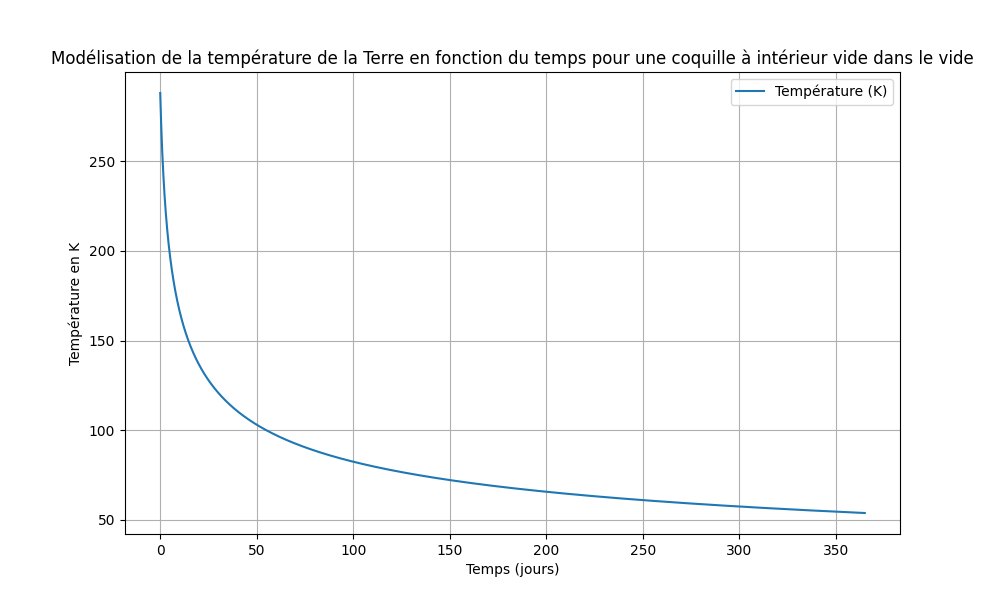
\includegraphics[width=0.8\linewidth]{../modele1/figures/modele1_coquille.png} 
\end{center}



\subsection{Critique du modèle}

\begin{itemize}
    \item Pas d’atmosphère, pas de rayonnement thermique reçu du Soleil, uniquement un transfert thermique émis par rayonnement.
    \item La Terre est assimilée à de d’eau.
    \item Température de la Terre subjective.
    \item Température du vide subjective.
    \item Épaisseur de la coquille arbitraire.
    \item On a supposé l'intérieur de la coquille vide, or cela implique un rayonnement à la fois vers l'intérieur et vers l'extérieur de la coquille.
\end{itemize}  

\newpage
\section{Modèle 2 : avec atmosphère}
\subsection{Boule d'eau avec atmosphère }
\addcontentsline{toc}{subsubsection}{Hypothèses}
\textbf{Hypothèses}
\begin{itemize}
    \item Terre assimilée à boule d'eau, de température \(T_{\text{Terre}}\) 
    \item  Atmosphère avec une température uniforme T 
    \item  Sans puissance solaire reçue  
    \item  Ignorance de la convection  
    \item \(c_m=c_{\text{m,Terre}}\sim c_{\text{m,eau}}\) 
    \item $T(t=0) = T_i$ \ \ \
$T(t \to +\infty) = T_0$
    \item La Terre ne rayonne pas
   
\end{itemize}
\vspace{0.5cm}
\subsubsection*{Schéma} 
\noindent\textcolor{gray}{\rule{\linewidth}{0.4pt}}

    
\begin{center}
  \input{modele2/figures/Schéma mathcha modèle 2.1.txt}
\end{center}
\noindent\textcolor{gray}{\rule{\linewidth}{0.4pt}}


\addcontentsline{toc}{subsubsection}{Équations de transfert thermique}
\textbf{Équations de transfert thermique}

On applique le premier principe au système \{ boule d'eau  \}

\begin{align*}
\delta Q &= C\, dT = -P_{\text{th,cond}} \cdot dt \\
\Rightarrow -\int \int \vec{j_{\text{th,cond}}}\, \vec{dS}\,dt = C\, dT \\
\Rightarrow -\int_{\theta=0}^\pi \int_{\phi=0}^{2\pi} h(T - T_0) \vec{e_{\text{r}}}\cdot r^2 \sin\theta\, d\theta\, d\varphi \vec{e_{\text{r}}}\, dt &=  C\, dT  \\
\Rightarrow -h(T - T_0) \cdot 4\pi\, dt &= C\, dT \\
\Rightarrow -T + T_0 = \frac{C}{h 4\pi} \frac{dT}{dt} \Rightarrow \frac{dT}{dt} &= -\frac{4\pi h}{C}(T - T_0)
\end{align*}

\vspace{0.5cm}

\addcontentsline{toc}{subsubsection}{Solution}
\textbf{Solution} 
$T(t) = T_0 + (T_i - T_0)e^{-kt}$ \quad avec $k = \frac{4\pi h}{C}$
\\
\bigskip

\addcontentsline{toc}{subsubsection}{Modélisation graphique}
\textbf{Modélisation graphique}
\begin{center}
  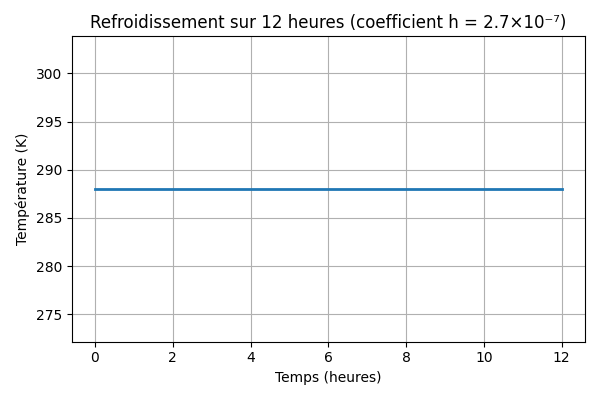
\includegraphics[width=0.8\linewidth]{../modele2/figures/modele2.png}
\end{center}
    
\vspace{1cm}
\subsection{Coquille assimilée à de l'eau avec atmosphère }
\addcontentsline{toc}{subsubsection}{Hypothèses}
\begin{itemize}
    \item On garde les hypothèses précédentes, en ajoutant l'atmosphère \end{itemize}
\vspace{1cm}
\addcontentsline{toc}{subsubsection}{Schéma}
\textbf{Schéma}
\\
\noindent\textcolor{gray}{\rule{\linewidth}{0.4pt}}

    
\begin{center}
  \input{modele2/figures/Schéma modèle 2.2 coquille.txt}
\end{center}
\noindent\textcolor{gray}{\rule{\linewidth}{0.4pt}}
\vspace{0.5cm}
\addcontentsline{toc}{subsubsection}{Modélisation graphique}
\textbf{Modélisation graphique}
\begin{center}
  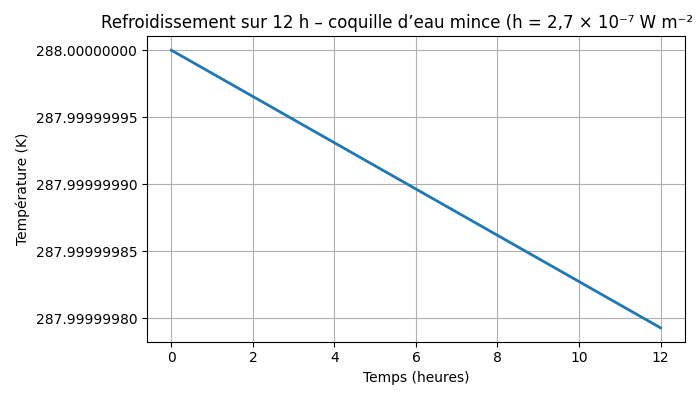
\includegraphics[width=0.8\linewidth]{../modele2/figures/modele2_coquille.png}
\end{center}
        


\subsection{Critique du modèle}

\begin{itemize}
    \item Température de la Terre subjective.
    \item Épaisseur de la coquille.
    \item Prise en compte de l’atmosphère donc utilisation de la loi de Newton :
    \begin{itemize}
        \item MAIS problème de définition de la couche limite puisqu’on ne souhaite pas prendre en compte la convection pour le moment.
    \end{itemize}
    \item Dans les codes \texttt{modele2\_coquille.py} et \texttt{modele2\_boule.py}, on a posé $h = \lambda_{\text{air}} / \delta$ avec $\lambda_{\text{air}} = 0{,}027 \, \mathrm{W/(K \cdot m)}$.
    \begin{itemize}
        \item On a pris $\delta = 100\, \mathrm{km}$ comme longueur de la couche limite pour ne pas se préoccuper de la convection avant la thermosphère (85 km – 600 km).
        \item Mais cette hypothèse ne semble pas pertinente, puisque la loi de Newton est adaptée à un modèle conducto-convectif.
        \item On peut donc prendre un $\delta$ plus raisonnable, de l’ordre de 50 cm.
    \end{itemize}
    \item Problème de définition de $T_0$ :
    \begin{itemize}
        \item Si on suit notre modèle, ce serait la température au-delà de la thermosphère.
        \item Or on a posé $T_0 = 273\, \mathrm{K}$ dans nos codes Python.
    \end{itemize}
\end{itemize}

\newpage
\section{Modèle 3 : intérieur de la coquille non vide }
\addcontentsline{toc}{subsubsection}{Hypothèses}
\textbf{Hypothèses}
\begin{itemize}
    \item Terre assimilée à une coquille d'eau avec intérieur non vide 
    \item  conduction entre centre de la terre et croûte (\(P_r\))
    \item  conduction entre croûte et air (\(P_{th,cond}\))
    \item  rayonnement de la croûte (\(P_{th,ray}\))
    \item On néglige le rayonnement de l'atmosphère
    \item $T(t=0) = T_i$ \ \ \
$T(t \to +\infty) = T_0$
     
\end{itemize}

\vspace{0.5cm}
\addcontentsline{toc}{subsubsection}{Schéma}
\textbf{Schéma}
\\
\noindent\textcolor{gray}{\rule{\linewidth}{0.4pt}}

    
\begin{center}
  \input{modele3/figures/Schéma modèle 3 coquille.txt}
\end{center}
\noindent\textcolor{gray}{\rule{\linewidth}{0.4pt}}

\addcontentsline{toc}{subsubsection}{Équations de transfert thermique}
\textbf{Équations de transfert thermique}

On applique le premier principe au système \{ coquille non vide  \}
\[
(-P_{\mathrm{th,cond}} - P_{\mathrm{th,ray}} + P_r)\,dt = C\,dT.
\]

\[
-\,h\bigl[T(r+dr)-T_0\bigr]\;4\pi
\;-\;4\pi\,\cdot (r+dr)^2\,\sigma\,T^4(r+dr)
\;-\;4\pi\,r^2\,\lambda\,\frac{\partial T}{\partial r}(r)
\;=\;C\,\frac{dT}{dt}.
\]

\medskip

Or au \(1^{er}\) ordre en \(dr\), \(r+dr\approx r\) :

\[
-4\pi\,h\bigl(T(r)-T_0\bigr)
\;-\;4\pi\,r^2\,\sigma\,T(r)^4
\;-\;4\pi\,r^2\,\lambda\,\frac{\partial T}{\partial r}(r)
\;=\;C\,\frac{dT}{dt}.
\]

\medskip

Avec
\[
P_{r}
= \iint\vec j_{\mathrm{thr}}\cdot d\vec S
= \iint -\lambda\,\vec{ \nabla } T\cdot d\vec S
= -\lambda
  \int_{0}^{\pi}\!\!\int_{0}^{2\pi}
    \frac{\partial T}{\partial r}\,\vec e_{r}\,
    r^2\sin\theta\;d\theta\,d\varphi\;\vec e_{r}
= -\lambda\,4\pi\,r^2\,\frac{\partial T}{\partial r}.
\]

\vspace{1cm}
\addcontentsline{toc}{subsubsection}{Modélisation graphique}
\textbf{Modélisation graphique}
    
    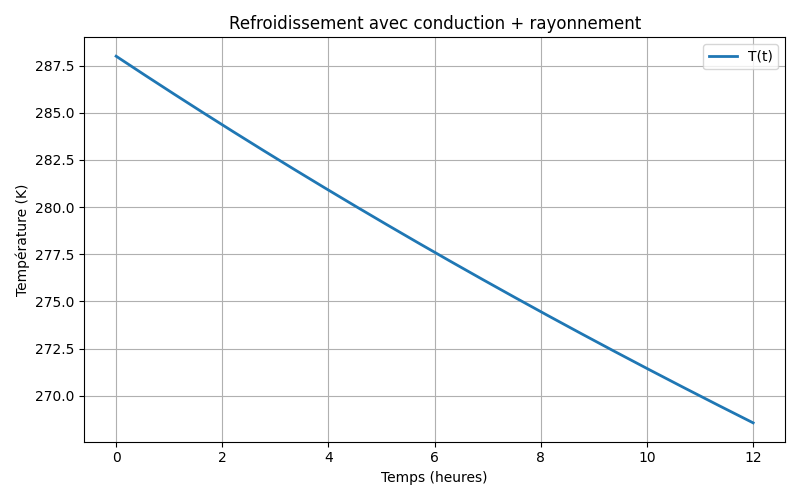
\includegraphics[width=0.8\linewidth]{../modele3/figures/modele3_coquille-conduction-rayonnement.png}    

\vspace{1cm}
\textbf{Critiques du modèle :}
\begin{itemize}
    \item La convection n’est pas prise en compte.
    \item dr doit être choisi de façon à ce que la température ne varie pas significativement.
    \item Problème de définition de $T_0$ :
    \begin{itemize}
        \item Si on suit notre modèle, ce serait la température au-delà de la thermosphère.
        \item Or on a posé $T_0 = 273\, \mathrm{K}$ dans nos codes Python. 
    
    \end{itemize}
\end{itemize}
\end{document}